
\documentclass[12pt,a4paper]{scrartcl}

\usepackage{amsmath}
\usepackage{fancyhdr}
\usepackage{times}
\usepackage[T1]{fontenc} 
\usepackage[latin1]{inputenc} 
\usepackage[ngerman]{babel}
\usepackage[right=3cm]{geometry}
\usepackage{listings}
\lstset{language=C,numbers=left,frame=single,breaklines=true,escapeinside={//\%}{\%}}
\usepackage{graphicx}
\usepackage{csvsimple}
\usepackage{float}

\parindent=0pt
\parskip=1em plus 2pt minus 1pt

\topskip-2cm
\textheight25cm
\pagestyle{fancy}
\fancyhead{}
\fancyfoot{}
\rhead{\thepage}

\begin{document}
\thispagestyle{empty}

\begin{center}
  \LARGE
  Praktische \"Ubungen - \\
  Experimentelle Hardwareprojekte \\
  \bigskip
  \Large 
  Versuchsprotokoll\\
  \small{\emph{\"Uberarbeitete Fassung vom 09. August 2018}}
\end{center}

\vspace{1em}
Versuch: G - GPU Programmierung

Versuchsdatum und -zeit:

G1: 30. Mai 2018, 14 - 17 Uhr / G2: 07: Juni 2018, 10 - 13 Uhr 

Betreuer: Ralf Seidler

\vspace{1em}
Name, Studiengang, Mat.-Nr.: Alexander K\"uhnle, B.Sc. Informatik, 165692

Email: alexander.kuehnle@uni-jena.de

\vspace{1em}
Name, Studiengang, Mat.-Nr.: Mark Umnus, B.Sc. Informatik, 167419

Email: mark.umnus@uni-jena.de

\vspace*{1cm}
%% \mbox{}\\
\hrule
\vspace*{1cm}
{\Large  Eigenst\"andigkeitserkl\"arung }
 
Hiermit versichern wir, dass wir das Protokoll selbstst\"andig verfasst
und keine anderen Quellen und Hilfsmittel als die angegebenen benutzt 
haben. Im Falle einer Zuwiderhandlung erkennen wir an, dass unser Protokoll 
als nicht bestanden bewertet wird und damit das Modul ``Experimentelle 
Hardwareprojekte'' als nicht bestanden bewertet wird. \\
Dar\"uberhinaus ist uns klar, dass jede Zuwiderhandlung ausnahmslos dem 
Rechtsamt der FSU gemeldet wird, woraus weitere Konsequenzen resultieren 
k\"onnen. \\

Unterschriften: \\ 
\hspace*{4cm} ........................................ 
\hspace{2cm} ........................................  \\

\hrule

\vspace*{0.3cm}
\textbf{Vom Betreuer auszuf\"ullen:}

Vorbereitung/Kolloquium:

Durchf\"uhrung:

Protokoll:

Gesamtbewertung:
\clearpage


% Hier geht das Protokoll los...

\section{Vorbereitung}
Um Berechnungen zu parallelisieren und dementsprechend auch enorm zu beschleunigen, werden heutzutage Multicore-Prozessoren verwendet.
Seit einigen Jahren gib es nun aber auch die M\"oglichkeit, Grafikkarten mit ihrer hohen Anzahl an Kernen f\"ur allgemeine Berechnungen zu verwenden.
Diese Eigenschaft namens \textit{General Purpose computing on Graphics Processing Units}, oder in kurz auch GPGPU, wird im Versuch G praktisch angewandt.

Mithilfe von bereitgestellten Nvidia-Grafikkarten, welche mit CUDA C programmiert werden k\"onnen, sollen typische Operationen der Bildbearbeitung implementiert werden.
Au\ss erdem soll die Performance der Implementierung analysiert werden.
Dazu sollen auch m\"ogliche Optimierungsm\"oglichkeiten der Codes gesucht, implementiert, analyisert und mit den urspr\"unglichen Werten verglichen werden.


\section{Vorgehensweise}
Uns wurden drei Server mit Nvidia-Grafikkarten zur Verf\"ugung gestellt, mit denen wir uns per \texttt{ssh} verbinden konnten.
Das Ziel des Praktikumsteils G1 ist es, eine Grafikkarte so zu programmieren, dass damit Bilder modifiziert werden k\"onnen.
Dazu wurden uns neben einem Testbild die folgenden Dateien zur Verf\"ugung gestellt:

\begin{description}
    \item [\texttt{cuda-kernels.cu}] Dieser Code wird auf der Grafikkarte ausgef\"uhrt, weswegen die Funktionalit\"at der Bildbearbeitung hier implementiert ist.
    \item [\texttt{cuda-host.cu}] Dieser Code wird auf dem Host ausgef\"uhrt. Er dient der Konfiguration und Ansteuerung der Grafikkarte.
    \item [\texttt{cuda-prak}] Dies ist das Executable, das aus dem Code entsteht.
\end{description}

Zudem lag ein Makefile bei, mit dem wir unsere Programme kompilieren und testen konnten.
Konkret sollte das Bild in der Helligkeit und im Kontrast angepasst, gespiegelt und in ein Graubild \"uberf\"uhrt werden.
Als komplexeste Aufgabe wurde final eine Kantendetektion angewendet.
Der Hostcode ist dabei zum gr\"o\ss ten Teil vorgegeben, der Devicecode muss im Laufe des Versuchs angepasst werden.

F\"ur den Praktikumsteil G2 wurden zus\"atzlich folgende Programme bereitgestellt:

\begin{description}
    \item [\texttt{cuda-kernels-int.cu}, \texttt{cuda-host-in.cu} und \texttt{cuda-prak-int}] Diese erf\"ullen die gleichen Aufgaben wie ihre oberen Gegenst\"ucke mit dem Unterschied, dass der \texttt{unsigned int}-Datentyp anstelle von \texttt{unsigned char} verwendet wird.
    \item [\texttt{cuda-nvvp}] Dieses Programm f\"uhrt eine Performance-Analyse f\"ur die verschiedenen in G1 implementierten Kernels durch.
    \item [\texttt{cuda-nvvp-int}] Hier sind die G2-Kernels das Ziel der Performance-Analyse.
    \item [\texttt{nvvp}] Der \emph{Nvidia Visual Profiler}, der detaillierte Einblicke in die Performance erm\"oglicht.
\end{description}

Gegenstand der Analyse waren die Anzahl an FLOPSs, der Datendurchsatz der Speicheroperationen und die Daten\"ubertragungsrate zwischen dem \textit{Device} und dem \textit{Host} analysiert werden.
Dazu wurde ebenfalls die Speichereffizienz auf dem globalen Speicher des \textit{Device} beobachtet.

Daraufhin sollten die G1-Kernelcodes optimiert werden, indem, wie bereits angesprochen, der Datentyp des Bildes ge\"andert wird.
Konkret wurde f\"ur die Farbwerte des Bildes den Datentyp \texttt{unsigned int} verwendet, um die Anzahl der Lade- und Speicheroperationen zu minimieren.
Zum Schluss wird der Code erneut mit dem Programm \texttt{cuda-nvvp} analysiert und mit den alten Werten verglichen.


\section{Erprobung}

\subsection{Aufgabenteil G1}
In diesem Aufgabenteil sind viele Zeilen Code entstanden, weswegen die vollst\"andigen Dateien im Anhang ab Seite \pageref{anhang} aufgef\"uhrt sind.
Dieser ist separat geklammert, um neben den Flie\ss{}text gelegt zu werden.

\subsubsection{Bild kopieren}
Diese Aufgabe diente als Einf\"uhrung, um mit dem Programmiermodell vertraut zu werden.
Au\ss erdem war damit Code gegeben, auf dem in den anderen Aufgaben aufgebaut werden konnte.
Die Kompilierung und die Ausf\"uhrung liefen wie erwartet.

\subsubsection{Helligkeit/Kontrast anpassen}
Die Ver\"anderung von Kontrast und Helligkeit eines Bildpunktes ist formal eine lineare Abbildung:

\begin{equation}\label{eq:linKernel}
    c_{neu} = \alpha \cdot c_{alt} + \beta
\end{equation}

Der Kontrast l\"asst sich anpassen, indem der Farbwert eines Bildpunktes mit einem Faktor $\alpha$ multipliziert wird.
Die Helligkeit wird per Addition mit $\beta$ angepasst.
Ver\"andert werden dabei nur die RGB-Werte von $c$, der Alphakanal bleibt unber\"uhrt.
Nach der Berechnung muss beachtet werden, dass der Bildpunkt $c_{neu}$ vom Typ \texttt{unsigned char} ist, was bedeutet, dass er Werte zwischen 0 und 255 annimmt.
Aus diesem Grund muss man kleinere oder gr\"o\ss ere Werte entsprechend anpassen.
In Listing \ref{a2.2} (Seite \pageref{a2.2}) geschah dies innerhalb der Zeilen \ref{line:linearStart} bis \ref{line:linearEnd}.
Zuerst wird die lineare Abbildung angewendet, dann werden die Werte auf das Intervall $[0,255]$ beschr\"ankt.
Abschlie\ss end ist ein Cast nach \texttt{unsigned char} n\"otig, da die berechneten Farbwerte vom Typ \texttt{float} sind.

\subsubsection{Bild spiegeln}
Nun sollte die linke Bildseite auf die rechte gespiegelt werden.
In dieser Hinsicht unterscheidet sich diese Aufgabe kaum von der ersten, es muss lediglich die Leseadresse angepasst werden.
Die Formeln daf\"ur waren in Einzelteilen bereits in der Versuchsvorbereitung gegeben.

\begin{align}
    adr & = (i + j \cdot width) \cdot 4 \nonumber\\
    c_{neu}(i,j) & =
        \begin{cases}
            c_{alt}(i,j) & \text{falls } i < width/2\\
            c_{alt}(width-i,j) & \text{sonst }
        \end{cases} \nonumber 
\end{align}

Substituiert man $c_{alt}(i,j)$ mit der Adressberechnung, so ergibt sich die Formel, die in Listing \ref{a2.3} verwendet wird:

\begin{equation} \label{eq:mirror}
    c_{neu}(i,j) =
        \begin{cases}
            (i + j \cdot width) \cdot 4 & \text{falls } i < width/2\\
            (width-i + j \cdot width) \cdot 4 & \text{sonst }
        \end{cases}
\end{equation}

Die betroffene Zeile \ref{line:mirror} im Code l\"asst die jeweilige Zeile im Bild (\texttt{j*width}) unver\"andert und w\"ahlt die Spalte von rechts nach links aus, wodurch der Spiegelungseffekt entsteht.
Der Faktor 4 ist notwendig, da jeder Bildpunkt aus 4 Werten (RGBA) besteht.

\subsubsection{Graubild erstellen}
In dieser Aufgabe sollte ein Graubild basierend auf dem Inputbild erstellt werden.
Mathematisch wird dabei jeder Kanal eines Bildpunkts im Ergebnisbild auf den Durchschnitt der Kanalwerte des Bildpunktes im Ausgangsbild gesetzt.
Dabei bleibt der Alphakanal wieder einmal unber\"uhrt.
Listing \ref{a2.4} zeigt den verwendeten Kernel, welcher sich nur geringf\"ugig vom Kopierkernel unterscheidet. 

Insgesamt war diese Aufgabe als Vorbereitung auf die n\"achste zu sehen, welche ein Graubild als Ausgangsbild ben\"otigt.

\subsubsection{Kantendetektion mit Sobel-Filter}
Eine detaillierte Erl\"auterung der Funktionsweise des Sobel-Filters findet sich in Abschnitt 1.1.5 der Versuchsbeschreibung.
Zusammengefasst werden zwei mit Sobel-Operatoren gewichtete Summen $g_x$ und $g_y$ von einem Bildpunkt und seinen 8 Nachbarn gebildet.
In einem zweiten Schritt wird die 2-Norm des Vektors ($g_x g_y$) gebildet, auf den Wertebereich der Farbkan\"ale gerundet und als Grauwert in das Ergebnisbild geschrieben, das hei\ss t derselbe Wert in jeden Farbkanal.
Per Definition erhalten Randpixel im Zielbild eine schwarze Farbe.
Unsere in diesem Versuch verwendete Implementierung ist in Listing \ref{a2.5old} zu sehen.
Diese enthielt jedoch einige Fehler -- auch bez\"uglich der Aufgabenstellung -- weswegen im Folgenden eine verbesserte Variante, n\"amlich Listing \ref{a2.5}  besprochen wird.
In Zeile \ref{line:sobelBoarder} wird gepr\"uft, ob der Bildpunkt ein Randpunkt ist und dementsprechend auf schwarz gesetzt werden muss.
Dies ist auch gleichzeitig der gr\"o\ss{}te Unterschied zur im Versuch benutzten Variante.
Hier gingen wir davon aus, dass mit der Bezeichnung "Rand" Bildpunkte au\ss{}erhalb des Bildes gemeint sind.
Die Folge war, dass innerhalb der gleich besprochenen Summation f\"ur jeden Pixel abgefragt werden musste, ob sein Nachbar au\ss{}erhalb des Bildes liegt.
In Listing \ref{a2.5old} ist dies in Zeile \ref{line:sobelOldIf} zu sehen.

Die Summen $g_x$ und $g_y$ werden durch die for-Schleifen realisiert.
Die Variablen \texttt{i\_new} und \texttt{j\_new} sind dabei die Koordinaten des Nachbarn, der gerade getrachtet wird.
Auf Basis dieser muss die Adresse im Ausgangsbild-Array berechnet und der jeweilige Farbwert geladen werden.
Es reicht an dieser Stelle vollkommen aus, nur einen Kanal zu laden, da das Ausgangsbild ein Graubild ist, welches die selben Farbwerte in allen Kan\"alen hat.
Wir haben zur leichteren Adressierung den Rotkanal gew\"ahlt.
In den Zeilen \ref{line:sobelSum}f wird dann die gewichtete Summation und in Zeile \ref{line:sobelNorm} wird anschlie\ss end die Normberechnung vorgenommen.
Hier ist ein zweiter Fehler im Originalcode zu finden:
Die \texttt{int}-Variable \texttt{bw} wird mit dem Wert aus der Wurzel beschrieben, der zum einen ein \texttt{float}-Wert ist und zum anderen au\ss{}erhalb des Wertebreichs f\"ur die Farbkan\"ale liegen kann.
In der \"uberarbeiteten Version wurde deswegen noch eine Korrektur wie im linearTransformKernel hinzugef\"ugt.
Bevor der Output geschrieben werden kann, muss der Wert des Alphakanals geladen werden, was in Zeile \ref{line:sobelLoadAlpha} geschieht.
Das Ergebnis des Sobel-Filters ist ein Graubild, weshalb wieder jeder Kanal denselben Wert erh\"alt.

Im zweiten Teil dieser Aufgabe musste noch der Host-Code geschrieben werden.
Dieser besitzt gro\ss{}e \"Ahnlichkeiten zu den \"ubrigen Host-Codes, jedoch gibt es den Unterschied, dass der Graubild- und der Sobel-Kernel nacheinander auf der GPU berechnet werden sollen, ohne dass das Zwischenergebnis auf den Host kopiert wird.
Dazu musste ein Zwischenspeicher auf der GPU reserviert werden, der als Ausgabe f\"ur den bwKernel und als Input f\"ur den sobelKernel verwendet wird.
Nach der Verwendung muss auch dieser Speicher freigegeben werden.
Auf Seite \pageref{a2.5host} ist das zugeh\"orige Listing \ref{a2.5host} zu finden.

\subsection{Aufgabenteil G2}
Dieser Aufgabenteil befasste sich mit der Analyse der zuvor geschriebenen Programme.
Zu diesem Zweck lag ein Bild in drei verschiedenen Gr\"o\ss{}en bereit, 1500x1000, 3000x2000 und 6000x4000 Pixel.
Daraus berechnen sich Speichergr\"o\ss{}en zwischen 5.7 und 91.55 MiB, welche sp\"ater ben\"otigt werden.
Die Ergebnisse des Versuchs sind im Anhang ab Seite \pageref{ergebnisse} zu finden.

\subsubsection{Performance-Analyse}
Mit Hilfe des Programms \texttt{cuda-nvvp} wurden die Zeiten gemessen, die die Kernel auf den verschiedenen Bildern gebraucht haben.
Zus\"atzlich wurden die Zeiten f\"ur die Organisation angezeigt, also f\"ur das Reservieren und Freigeben von Speicher und f\"ur das \"Ubertragen der Daten.
Genaue Zahlen sind in den Tabellen ab Seite pageref{rohdaten} aufgef\"uhrt.
Die Durchschnittszeiten der Messungen sind auf Abbildung \ref{fig:timesize} zu sehen.
Hier sieht man deutlich, dass k\"urzere Zeiten erreicht werden, wenn die Threadkonfiguration gr\"o\ss{}ere Bl\"ocke vorsieht.
Das gilt f\"ur alle Kernel.
Gleichzeitig erfolgen die Berechnungen auf dem 6000x4000-Bild bei optimaler Konfiguration schneller als die auf dem kleinsten Bild bei schlechter Konfiguration.
Der Speedup-Faktor zwischen der 1x1- und der besten Konfiguration liegt jeweils bei ungef\"ahr 50 und ist relativ unabh\"angig von der Bildgr\"o\ss{}e.

Auf Abbildung \ref{fig:timekernel} kann man die Verbesserung der einzelnen Kernel auf dem gleichen Bild betrachten, w\"ahrend die Blockkonfigurationen wieder auf der x-Achse abgetragen sind.
Die anderen Bildgr\"o\ss{}en zeigen ganz \"ahnliche Verl\"aufe.
Auch hier sieht man, dass es f\"ur jeden einzelnen Kernel vorteilhaft ist, mit einer gro\ss{}en Konfiguration angewendet zu werden.
Interessant an den zugeh\"origen Daten in Tabelle \ref{tab:messwertemedium} ist, dass der copyKernel verh\"altnism\"a\ss{}ig langsam ist, obwohl er kaum etwas zu rechnen hat.
Allerdings macht ihn genau das langsam:
Grafikkarten k\"onnen gut rechnen, Speicheroperationen sind jedoch langsam und blockieren sich gegenseitig, wenn zu viele gleichzeitig laufen.

F\"ur das \"Ubertragen der Daten wurden Zeiten von 1.363ms f\"ur das kleine Bild und 19.5ms f\"ur das gr\"o\ss{}te Bild gemessen.
Gem\"a\ss{} der Formel

\begin{align}\label{form:bandbreite}
    \text{Speicherbandbreite}[\frac{Byte}{s}] = \frac{\text{Datenmenge}[Byte]}{\text{Zeit}[s]}
\end{align}

ergeben sich Speicherbandbreiten zwischen 4.0997 und 4.58 GiB/s.
Diese sind f\"ur die gleiche Bildgr\"o\ss{}e auch sehr \"ahnlich, wenn man Host->Device und Device->Host vergleicht.

In der performantesten Konfiguration, also mit 24MP-Eingabebild und 32x32-Threadkonfiguration, erreichen die Kernel die in Tabelle \ref{tab:perf} dargestellten Werte.
Die Berechnung der Performance erfolgte analog zu Formel (\ref{form:bandbreite}) in $\frac{FLOPS}{s}$.

\begin{table}[h]
    \centering
    \begin{tabular}{l|l|l}
    \hline
    Kernel & Performance in GFLOPS/s & Speicherbandbreite in GiB/s \\
    \hline
    copyKernel & --                  & 31.463 \\
    linearTransformKernel & 25.855   & 31.54 \\
    mirrorKernel & --                & 39.278 \\
    bwKernel & 12.717                & 31.584 \\
    sobelKernel & 123.806            & 40.356 \\
    \hline
    \end{tabular}
    \caption{\"Ubersicht der Werte der Kernel in der besten Konfiguration}
    \label{tab:perf}
\end{table}

F\"ur den copyKernel und den mirrorKernel haben wir keine FLOPS/s angegeben, da keine FP-Arithmetik verwendet wird.
Beim linearTransformKernel treten 6 FLOPS auf, beim bwKernel 3 und beim sobelKernel 40.
Die Speicheroperationen sind bei jedem Kernel 8 (4 zum Laden, 4 zum Speichern), au\ss{}er beim sobelKernel, wo die Anzahl der Speicheroperationen in unserer Fassung zwischen 9 und 14\footnote{definitiv den Alphakanal laden, 4 Kan\"ale schreiben und in den Schleifen 4 bis 9 laden} lag, je nachdem, ob der betrachtete Pixel in der Mitte, an der Kante oder sogar Ecke des Bildes liegt.
In der Tabelle \ref{tab:perf} haben wir mit 14 gerechnet, weil das auf den gr\"o\ss{}ten Teil der Pixel zutrifft.

Um noch genauere Informationen zu erhalten, haben wir den Nvidia Visual Profiler genutzt.
Auf Abbildung 3 sieht man, dass die Load und Store Efficiencys mit 21.8 bzw. 25 Prozent sehr gering sind.
Das hat den Grund, dass jeder Thread 4 Werte aus dem Global Memory laden muss, etwas berechnet und 4 Werte danach wieder zur\"uckschreiben muss.
Im folgenden Abschnitt betrachtet man die Bilder als Integer-Arrays, um pro Pixel nur noch einen Wert laden zu m\"ussen.

\subsubsection{Performance-Steigerung}
Um die Berechnungen fast 1:1 beibehalten zu k\"onnen, haben wir Makros definiert, wie es in der Versuchsbeschreibung auf den Seiten 15 und 16 beschrieben ist.
Zusammengefasst trennt man den geladenen Integerwert in Bytes auf und f\"ugt ihn nach der Berechnung wieder zusammen.
Dabei werden die Shiftoperationen genutzt.
Es musste zudem beachtet werden, dass die Adressen zweier aufeinanderfolgender Pixel nun nicht mehr um vier auseinanderliegen, sondern nur noch um eins.
Als Beispiel f\"ur diese \"Uberarbeitung haben wir den Integer-sobelKernel im Anhang dieses Protokolls in Listing \ref{a3.2} gezeigt, da hier alle \"Anderungen konzeptionell vorhanden sind.
Der Hostcode musste ebenfalls angepasst werden, um die Bilder als Integer-Arrays zu behandeln.

Die anschlie\ss{}end mit \texttt{cuda-nvvp-int} gemessenen Werte sind in Tabelle \ref{tab:perf-int} aufgef\"uhrt.

\begin{table}[h]
    \centering
    \begin{tabular}{l|l|l}
    \hline
    Kernel & Performance in GFLOPS/s & Speicherbandbreite in GiB/s \\
    \hline
    copyKernel & --                  & 31.86  \\
    linearTransformKernel & 25.668   & 31.874 \\
    mirrorKernel & --                & 44.981 \\
    bwKernel & 12.869                & 31.961 \\
    sobelKernel & 129.152            & 42.099 \\
    \hline
    \end{tabular}
    \caption{\"Ubersicht der Werte der Integer-Kernel in der besten Konfiguration}
    \label{tab:perf-int}
\end{table}

Die Ergebnisse sind erwartungsgem\"a\ss{} besser ausgefallen als die mit der char-Verwendung.
Vor allem der sobelKernel, der die meisten Ladeoperationen hat, profitiert davon.
Das sieht man auch auf Abbildung \ref{fig:sobelint}, bei der sich die Store Efficiency auf ganze 99.8\% erh\"oht hat.
Die Load Efficiency hat sich ebenfalls erh\"oht, wenn auch nicht so stark.
Im sobelKernel sind viel mehr Ladeoperationen n\"otig, die nur einen Farbkanal ben\"otigen, sodass der Effekt nicht so stark ausf\"allt.


\section{Schlussfolgerungen}
In diesem Versuch wurde gezeigt, dass GPUs m\"achtige Werkzeuge sind, die man aber korrekt handhaben muss, um das meiste Potenzial aus ihnen herauszuholen.
Vor allem die geringe Speicherbandbreite zwischen Host und Device bzw. zwischen dem Global Memory und den Recheneinheiten begrenzt die Geschwindigkeit von oben.
Aus diesem Grund sollte man haupts\"achlich solche Teile auf die GPU auslagern, die viel rechnen und wenige Speicherzugriffe ben\"otigen.
Zus\"atzlich kann man die Berechnungen beschleunigen, indem man die Konfiguration der Bl\"ocke und Threads den Daten anpasst.
Insbesondere zu kleine Blockkonfigurationen sollten vermieden werden, da sonst der Overhead gegen\"uber der effektiven Nutzung zu hoch ist.

\newpage
\section{Anhang}
\appendix
\label{anhang}

\section{Programme}
\lstinputlisting[firstline=24,lastline=59,caption=linearTransformKernel in \texttt{cuda-kernels.cu},label=a2.2]{cuda-kernels.cu} \newpage
\lstinputlisting[firstline=61,lastline=89,caption=mirrorKernel in \texttt{cuda-kernels.cu},label=a2.3]{cuda-kernels.cu} \newpage
\lstinputlisting[firstline=91,lastline=115,caption=bwKernel in \texttt{cuda-kernels.cu},label=a2.4]{cuda-kernels.cu} \newpage
\lstinputlisting[firstline=117,lastline=161,caption=sobelKernel in \texttt{cuda-kernels.cu},label=a2.5old]{cuda-kernels.cu} \newpage
\lstinputlisting[firstline=1,lastline=45,caption=verbesserter sobelKernel,label=a2.5]{cuda-kernels-better.cu} \newpage
\lstinputlisting[firstline=65,lastline=81,caption=sobelCuda in \texttt{cuda-host.cu},label=a2.5host]{cuda-host.cu} \newpage
\lstinputlisting[firstline=119,lastline=160,caption=sobelKernel in \texttt{cuda-kernels-int.cu},label=a3.2]{cuda-kernels-int.cu}

\section{Analyseergebnisse}
\label{ergebnisse}
\begin{figure}[H]
    \caption{}
    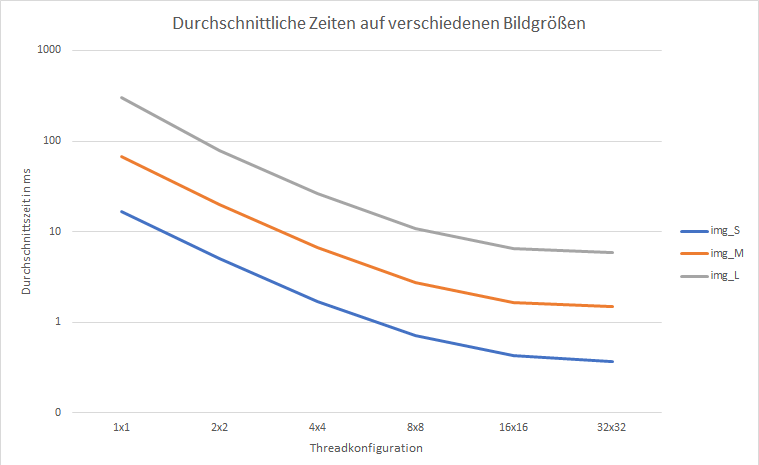
\includegraphics[width=0.9\textwidth]{times(size).png}
    \label{fig:timesize}
\end{figure}

\begin{figure}[H]
    \caption{}
    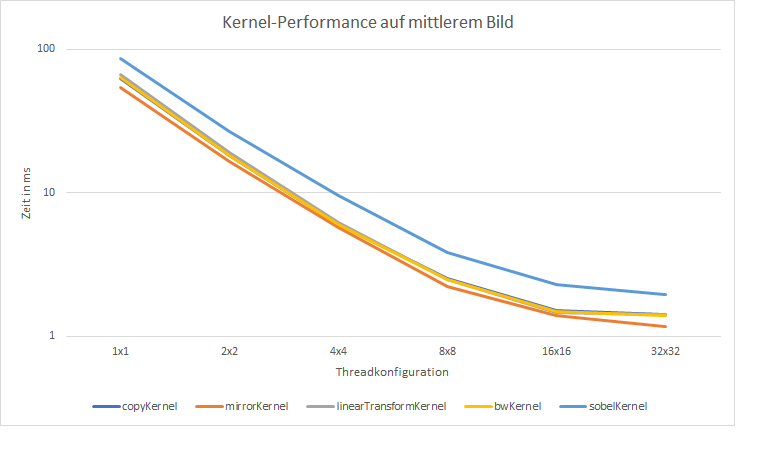
\includegraphics[width=0.9\textwidth]{times(kernel).png}
    \label{fig:timekernel}
\end{figure}

\begin{figure}[H]
    \caption{Nvidia Visual Profiler angewendet auf cuda-prak}
    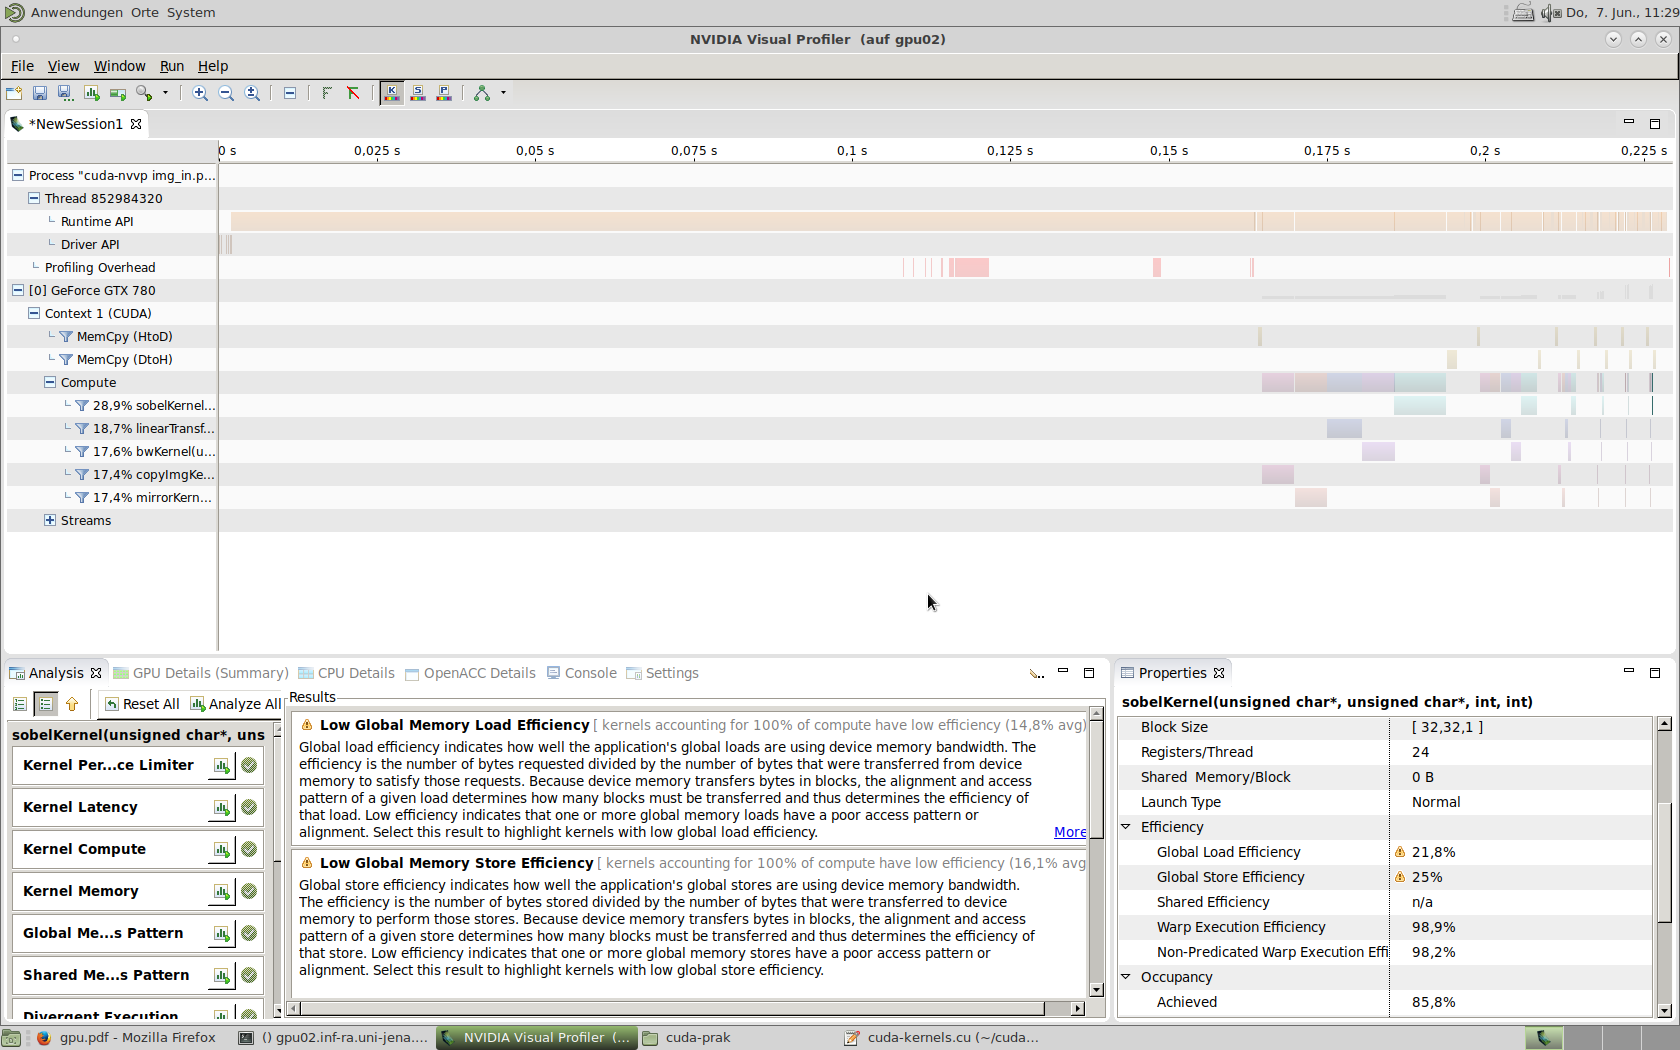
\includegraphics[width=0.9\textwidth]{Sobel_Char_Efficiency.png}
    \label{fig:sobelchar}
\end{figure}

\begin{figure}[H]
    \caption{Nvidia Visual Profiler angewendet auf cuda-prak-int}
    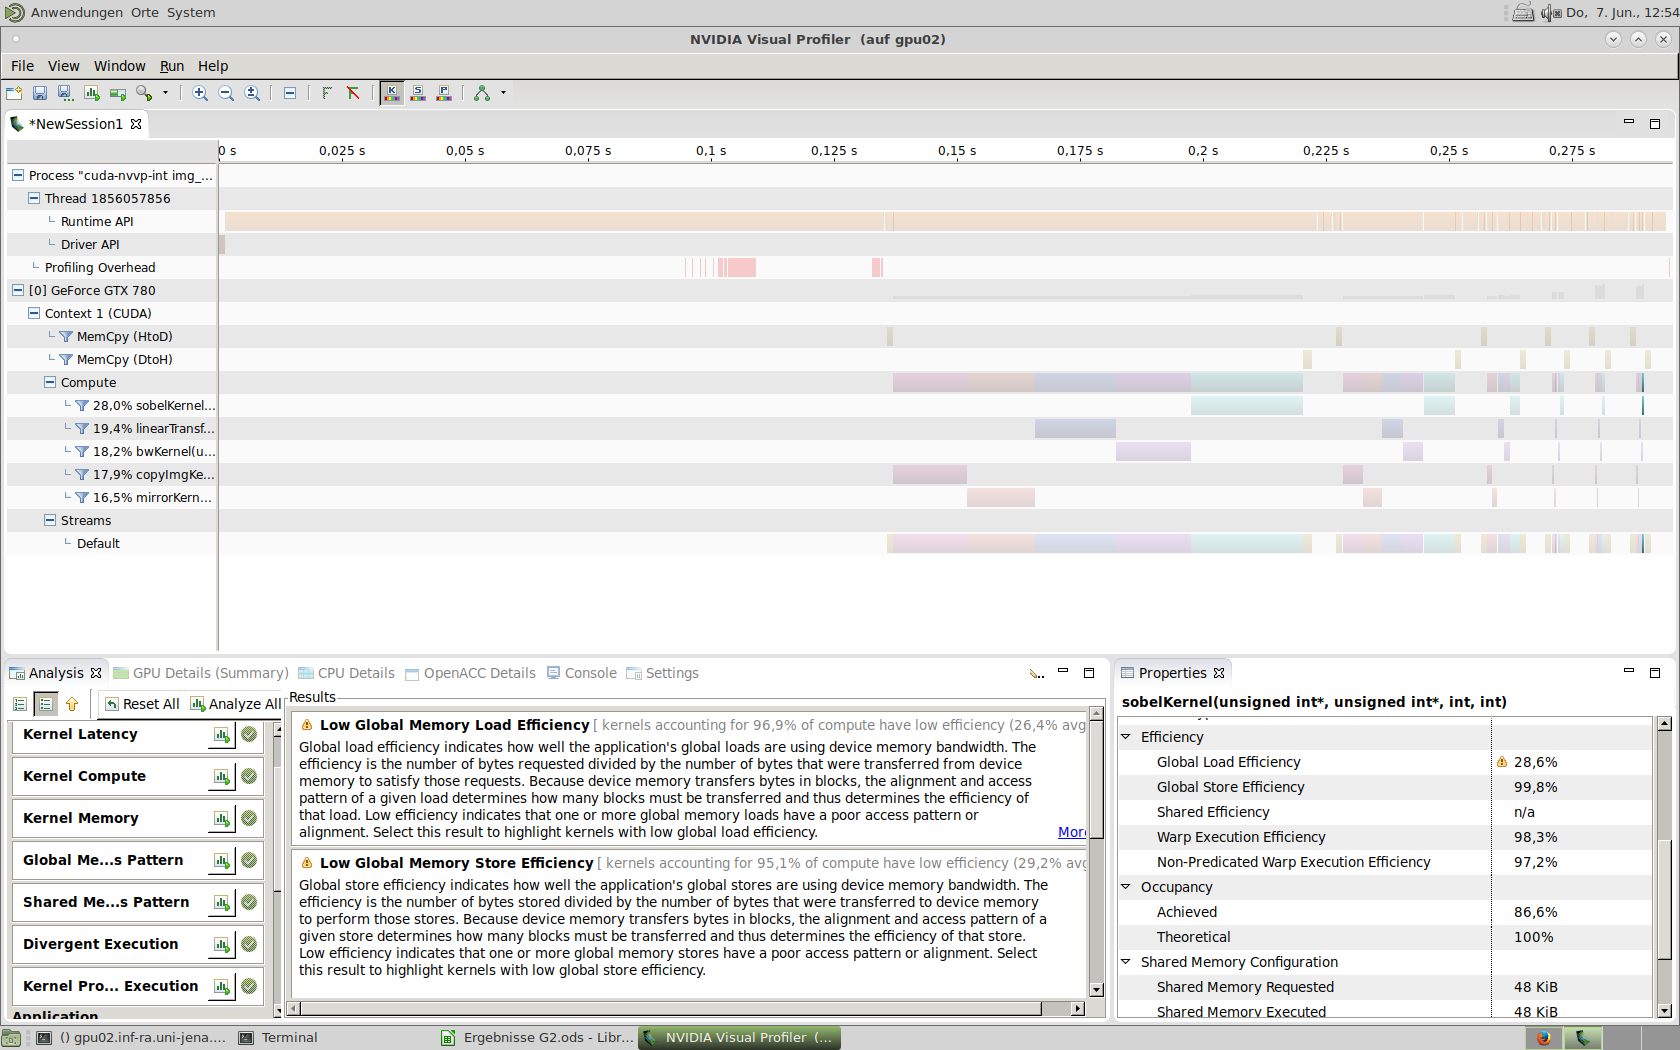
\includegraphics[width=0.9\textwidth]{Sobel_Int_Efficiency.png}
    \label{fig:sobelint}
\end{figure}

\section{Rohdaten}
\label{rohdaten}
\begin{table}[H]
    \centering
    \csvautotabular{smallimage-char.csv}
    \caption{char-Messwerte auf kleinem Bild in ms}
    \label{tab:messwerteklein}
\end{table}

\begin{table}[H]
    \centering
    \csvautotabular{mediumimage-char.csv}
    \caption{char-Messwerte auf mittlerem Bild in ms}
    \label{tab:messwertemedium}
\end{table}

\begin{table}[H]
    \centering
    \csvautotabular{largeimage-char.csv}
    \caption{char-Messwerte auf gro\ss{}em Bild in ms}
    \label{tab:messwertelarge}
\end{table}

\begin{table}[H]
    \centering
    \csvautotabular{smallimage-int.csv}
    \caption{int-Messwerte auf kleinem Bild in ms}
    \label{tab:messwerteklein-int}
\end{table}

\begin{table}[H]
    \centering
    \csvautotabular{mediumimage-int.csv}
    \caption{int-Messwerte auf mittlerem Bild in ms}
    \label{tab:messwertemediumint-}
\end{table}

\begin{table}[H]
    \centering
    \csvautotabular{largeimage-int.csv}
    \caption{int-Messwerte auf gro\ss{}em Bild in ms}
    \label{tab:messwertelarge-int}
\end{table}

\begin{table}[H]
    \centering
    \csvautotabular{memtime.csv}
    \caption{Memory Timings in Abh\"angigkeit von der Bildgr\"o\ss{}e}
    \label{tab:memtimings}
\end{table}


\end{document}
